% 2013 天津卷文科第 17 题：三棱柱 ABC-A1B1C1，侧棱 A1A ⊥ 底面 ABC，各棱长均相等，
% D、E、F 分别为 AB、BC、A1C1 的中点。前面 A1C1CA 可见，A1C、FE、A1D 为辅助线。
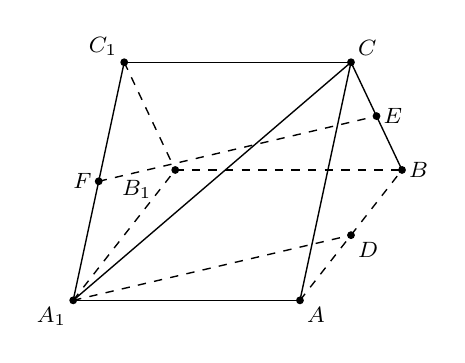
\begin{tikzpicture}[font=\footnotesize, line width=0.5pt, scale=0.72,
  dot/.style={circle, fill=black, inner sep=1.0pt}]
  \coordinate (A1) at (0,0);
  \coordinate (A)  at (4,0);
  \coordinate (C1) at (0.9,4.2);
  \coordinate (C)  at (4.9,4.2);
  \coordinate (B)  at (5.8,2.3);
  \coordinate (B1) at (1.8,2.3);
  \coordinate (D)  at (4.9,1.15);
  \coordinate (E)  at (5.35,3.25);
  \coordinate (F)  at (0.45,2.1);
  % 可见棱与可见面上的辅助线
  \draw (A1) -- (A);
  \draw (A) -- (C);
  \draw (C) -- (C1);
  \draw (C1) -- (A1);
  \draw (C) -- (B);
  \draw (A1) -- (C);
  % 不可见棱与内部辅助线
  \draw[dashed] (A) -- (B);
  \draw[dashed] (B1) -- (B);
  \draw[dashed] (C1) -- (B1);
  \draw[dashed] (A1) -- (B1);
  \draw[dashed] (A1) -- (D);
  \draw[dashed] (F) -- (E);
  \foreach \p in {A,B,C,A1,B1,C1,D,E,F} \node[dot] at (\p) {};
  \node[above left=-1pt] at (C1) {$C_1$};
  \node[above right=-1pt] at (C) {$C$};
  \node[below left=-1pt] at (A1) {$A_1$};
  \node[below right=-1pt] at (A) {$A$};
  \node[right=-1pt] at (B) {$B$};
  \node[left=5pt, yshift=-7pt] at (B1) {$B_1$};
  \node[below right=-1pt] at (D) {$D$};
  \node[right=-1pt] at (E) {$E$};
  \node[left=-1pt] at (F) {$F$};
\end{tikzpicture}
